\documentclass[11pt]{article}
\usepackage[utf8x]{inputenc}
\usepackage[english]{babel}
\usepackage{graphicx}
\usepackage{wrapfig}
\usepackage[margin=1.5cm, tmargin=1.5cm]{geometry}
\usepackage{color}
\usepackage{hyperref}
\usepackage{array}

\begin{document}
 \bibliographystyle{plain}%Choose a bibliograhpic style
\title{Network training}
\date{Fall 2014}
\author{Maël Auzias}
\maketitle

%\tableofcontents
%\pagebreak


\section{Introduction}
\subsection{Classification}
Give a concrete example of each of the following kinds of networks (name some devices):
  \begin{enumerate}
    \item BAN,
    \item PAN,
    \item LAN,
    \item WAN.
  \end{enumerate}

\subsection{Topologies}
Give a concrete example of each of the following network topologies:
  \begin{enumerate}
    \item Bus,
    \item Star,
    \item Fully connected.
  \end{enumerate}

\subsection{TCP connection}
According to TCP (\color{blue}\href{http://tools.ietf.org/html/rfc761}{RFC761 (January 1980)}) \color{black}, what are the sequences used in order to establish a connection between two hosts?

\subsection{TCP or UDP?}
\subsubsection{Sensors}
You are creating a network application using sensors. The sensors can receive requests to change their settings (rate of measurement, range...) and they continuously send their measurements.
  \begin{enumerate}
    \item Should request packets (settings) be sent with UDP or TCP? Why?
    \item Should measurement packets be sent with UDP or TCP? Why?
  \end{enumerate}
\subsubsection{Website}
Does HTTP (\color{blue}\href{http://tools.ietf.org/html/rfc2616}{RFC2616 (June 1999)}) \color{black} rely on TCP or UDP? Why?

\subsection{FTP}
\subsubsection{Is FTP secure?}
According to the file \color{blue}\href{http://teaching.auzias.net/db/ftp-connect.pcap}{ftp-connect.pcap} \color{black} is FTP secure? What could you do to use it more securely?
\subsubsection{FTP and TCP}
According to the file \color{blue}\href{http://teaching.auzias.net/db/ftp-disconnect.pcap}{ftp-disconnect.pcap} \color{black} does FTP respect the TCP protocol to close a connection?

\subsection{DNS}
\subsubsection{Some news}
According to the file \color{blue}\href{http://teaching.auzias.net/db/nslookup.pcap}{nslookup.pcap} \color{black} what is:
  \begin{enumerate}
    \item the DNS server?
    \item the domain name for which the IP address is needed?
    \item the IP address of the domain if any?
  \end{enumerate}n
\subsubsection{Which one?}
According to the file \color{blue}\href{http://teaching.auzias.net/db/nslookup-whoseone.com.pcap}{nslookup-whoseone.com.pcap} \color{black} what is:
  \begin{enumerate}
    \item the DNS server?
    \item the domain name for which the IP address is needed?
    \item the IP address of the domain if any?
  \end{enumerate}

\subsection{Ping-pong}
\subsubsection{Are you there?}
According to the file \color{blue}\href{http://teaching.auzias.net/db/ping.pcap}{ping.pcap} \color{black}:
  \begin{enumerate}
    \item what is the node 127.0.0.1 doing?
    \item Is the node 127.0.0.2 on the network?
  \end{enumerate}
\subsubsection{Who has this IP?}
According to the file \color{blue}\href{http://teaching.auzias.net/db/arp.pcap}{arp.pcap} \color{black} and to ARP (\color{blue}\href{http://tools.ietf.org/html/rfc826}{RFC826 (November 1982)})\color{black}. What is the source trying to do? What is ARP used for? If ever a host does not respond to ping (i.e., for security reasons), how could you check if the host is up anyway ?


%%%%%%%%%%%%%%%%%%%%%%%%
%%      Layer 1       %%
%%%%%%%%%%%%%%%%%%%%%%%%
\section{Physical layer}
\subsection{General}
\subsubsection{Aims}
What are the layer-1 goals?
\subsubsection{Name it}
What is the common (\emph{commercial}) name of:
  \begin{enumerate}
    \item IEEE 802.11
    \item IEEE 802.15.1
    \item IEEE 802.15.4
  \end{enumerate}
What is IEEE 802.15 related to? What does WPAN stand for?

\subsection{Encoding, encrypting, decoding}
It is important to know what are the differences between encoding and encryption. The following questions are related to theses subjects.
\subsubsection{Encrypt?}
What are the differences between encoding and encryption?\\
What are the two main kinds of encryption? Their advantages?\\
Name three well known cryptographic methods and three well known encoding methods.

\subsubsection{Encode it}
The string \verb$"Zp"$ (which does not mean anything but has a nice binary value) is, according to ASCII, \verb$0x5a70$. Encode it using:
  \begin{enumerate}
    \item Multi-Level Transmit
    \item Alternate Mark Inversion
    \item Manchester (or differential Manchester)
    \item Biphase Mark Code
  \end{enumerate}

\subsubsection{Decode it}
What are the ASCII characters of theses images:
  \begin{figure}[h]
    \centering
    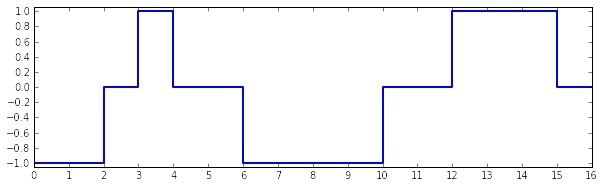
\includegraphics[height=3cm]{../slides/imgs/MLT3:).jpg}
    \caption{MLT3 encoded}
    \label{fig:mlt3}
  \end{figure}
  \begin{figure}[h]
    \centering
    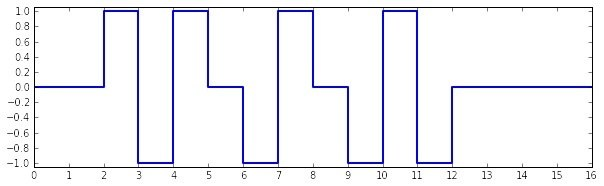
\includegraphics[height=3cm]{../slides/imgs/AMI;p.jpg}
    \caption{AMI encoded}
    \label{fig:ami}
  \end{figure}

\subsection{For\emph{Oh}For error}
\subsubsection{Calculate it}
What would be the output of the binary: \verb$0b0011 0000 1110 1001$ using the error detection methods:
  \begin{enumerate}
    \item Repetition (2)
    \item Parity (odd)
    \item Parity (even)
    \item Checksum (over 4 bit)
    \item MD5 hash
  \end{enumerate}

\subsubsection{Validate it}
Are theses received data correct? NB: detection values are in square brackets.
  \begin{enumerate}
    \item Using repetition (2), was received: \verb$0b0011 0011 0000 0000 1110 1001 1001 1001$
    \item Using parity (odd), was received: \verb$0b1011[1] 1010[0] 1100[1] 0111[1]$
    \item Using parity (even), was received: \verb$0b1011[1] 1010[0] 1100[1] 0111[1]$
    \item Using checksum (over 4 bit), was received: \verb$0b0011 0111 0010 0010 1110 1001 1101 1001 [1011]$
    \item Using MD5, the string was received (without the quotes): \verb$"that's way too long..."$ the md5 sum: \verb$[3be37cad170213a8ad936c0640e3238b]$
  \end{enumerate}


\subsubsection{Correct it}
By using MDPC (Multidimensional parity-check code) the data received are: \verb$0x01 09 0e 06 03 09 0b 0c$. Are the data correct? What would be the correction? \\
  \begin{figure}[h]
    \centering
    \begin{tabular}{cc|c}
      0x01 & 0x09 & 0x0e \\
      0x06 & 0x03 & 0x09 \\ \hline
      0x0b & 0x0c &
    \end{tabular}
    \caption{Data received with MDPC}
    \label{fig:ami}
  \end{figure}

\subsubsection{Half or full?}
What is the difference between half and full duplex medium?

%%%%%%%%%%%%%%%%%%%%%%%%
%%      Layer 2       %%
%%%%%%%%%%%%%%%%%%%%%%%%
\section{Data layer}
\subsection{General}
\subsubsection{Aims?}
What are the main objectives of the data layer?
\subsubsection{Composition}
What are the sublayer of the data layer?
\subsection{Ethernet packet decoding}
According to the packet \ref{fig:arp_req_ex}, which machine tried to ping which machine? Give MAC and IP address of both machines.
  \begin{figure}[h]
  \centering
  \resizebox{16cm}{!} {
    \begin{tabular}{lcccccccccccccccc}
      \textbf{0000} & ff & ff & ff & ff & ff & ff & 00 & 1b & 11 & 09 & aa & 88 & 08 & 06 & 00 & 01 \\
      \textbf{0010} & 08 & 00 & 06 & 04 & 00 & 01 & 00 & 1b & 11 & 09 & aa & 88 & c0 & a8 & 00 & 3b \\
      \textbf{0020} & 00 & 00 & 00 & 00 & 00 & 00 & c0 & a8 & 00 & 3c \\
    \end{tabular}
  }
  \caption{Layer 2 packet}
  \label{fig:arp_req_ex}
  \end{figure}
\subsection{Ping}
For security reasons, the administrator of a machine disable the ping response. By knowing its MAC address, how can you assure that this host is up or not (assuming no other security rules on the machine)?
\subsection{CSMA/CA}
What does this acronym stand for? What and how is it used for? Is there any differences for the CSMA/CA between half and full duplex medium?

%%%%%%%%%%%%%%%%%%%%%%%%
%%      Layer 3       %%
%%%%%%%%%%%%%%%%%%%%%%%%
\section{Network layer}
\subsection{General}
\subsubsection{Aims?}
\begin{enumerate}
  \item What are the main objectives of the network layer?
  \item What are the two main objectives of host addressing?
  \item Does this layer use reliable communication? What is the difference between end-to-end packet transmission layer-2 and layer-3?
  \item What is the routing used for? What is "load balancing"?
\end{enumerate}
\subsubsection{Adressing}
\begin{enumerate}
  \item How many bits does an IP address have?
  \item What are the two part of an IP address?
  \item How many bits is each part? What does determine it?
  \item How is a mask constituted?
  \item How many addresses and nodes does theses mask allow: 31, 30, 24, 16, 8, 4?
  \item What are the specification of network and broadcast addresses?
  \item What are the first and last \textbf{nodes} IP addresses of theses networks:
    \begin{itemize}
      \item 192.168.2.0/24
      \item 192.168.2.0/23
      \item 172.13.0.0/16
      \item 10.0.1.0/31
      \item 10.0.2.0/30
    \end{itemize}
  \item What are the classes of theses IP addresses?
    \begin{itemize}
      \item 1.2.3.4
      \item 192.168.2.35
      \item 8.8.8.8
      \item 208.67.222.222
      \item 208.67.220.220
      \item 176.34.131.233
      \item 127.192.168.1
      \item 224.0.0.2
      \item 0.0.0.0
    \end{itemize}
\end{enumerate}

\subsection{Designing}
\subsubsection{Subnetworks}
Starting from the 192.168.0.0 IP address, calculate the subnet masks, subnetwork IP address, first node IP address, last node IP address and broadcast addresses for theses networks:
\begin{itemize}
  \item 29 hosts,
  \item 60 hosts,
  \item 121 hosts.
\end{itemize}
Theses network are all on the same CIDR 192.168.0.0/24.

\subsubsection{Inter-network}
A inter-network is as follow:
\begin{itemize}
  \item With two routers (A and B) within the subnetwork having 10.0.0.0 has IP address.
  \item Router A has a subnetwork n1, with 40 hosts, having 192.168.3.64 IP address.
  \item Router A has a subnetwork n2, with 10 hosts, having 192.168.3.144 IP address.
  \item Router B has a subnetwork n3, with 1500 hosts, having 176.16.0.0 IP address.
  \item Router B has a subnetwork n4, with 30 hosts, having 176.31.25.224 IP address.
\end{itemize}

How many different subnetworks are in this network?\\
How many NIC do the routers A and B have?\\
Draw the schema of the network?\\
Design, using the best subnet mask for each subnet (subnet masks, subnetwork IP address, first node IP address, last node IP address, broadcast address).

\subsection{CIDR}
\subsubsection{Subnetworks}
The following networks are in a routing-table. Is it possible to combine routes? How? Which ones?
\begin{figure}[h]
  \centering
  \resizebox{10cm}{!} {
    \begin{tabular}{lllr}
      \textbf{Destination} & \textbf{Gateway} & \textbf{Genmask} & \textbf{Iface} \\ \hline
      192.168.0.0   & 10.0.0.2 & 255.255.255.128 & E0 \\
      130.1.2.0     & 10.0.0.6 & 255.255.0.0     & E1 \\
      192.168.1.112 & 10.0.0.2 & 255.255.255.240 & E0 \\
      192.168.3.0   & 10.0.0.2 & 255.255.248.0   & E0 \\
      192.168.5.0   & 10.0.0.6 & 255.255.248.0   & E1 \\
    \end{tabular}
  }
  \caption{Routing table example}
  \label{fig:rting-tbl}
\end{figure}
What is the important information that is missing to route?
\subsection{Routing}
\subsubsection{New route}
A router just got a new IP address: 57.6.96.0/21, 57.6.104.0/21, 57.6.112.0/21, 57.6.120.0/21. If the routes uses the same NIC, can they be summarized?%57.6.96.0/19
\subsubsection{New network}
A router has a route for the range 29.18.0.0 to 29.18.128.255 into the route 29.18.0.0/17. A new 1024-addresses network, from 29.18.60.0 to 29.18.63.255, got advertise on a new interface of the router. Should the CIDR be spread out?%Nope, the new route is 29.18.0.0/22, if a packet comes for this network, the submask is bigger than the 29.18.0.0/17, so the better match will be for the new route.
\subsubsection{Next hop?}
A router has the routing table:
  \begin{figure}[h]
  \centering
    \begin{tabular}{ll}
      \textbf{Address/mask} & Next hop \\ \hline
      135.46.56.0/22        & Iface 0  \\
      135.46.60.0/22        & Iface 1  \\
      192.53.40.0/23        & Router 1 \\
      0.0.0.0               & Router 2 \\ \hline
    \end{tabular}
  \caption{Routing table}
  \end{figure}
What will the router do with packets being destined to:
\begin{itemize}
  \item 135.46.63.10  %iface1
  \item 135.46.57.14  %iface0
  \item 135.46.52.2   %router 2
  \item 192.53.40.7   %router 1
  \item 192.53.56.7   %router 2
\end{itemize}
\subsubsection{Two or one router?}
Lot of firm uses two routers in case of one crashes. Is the NAT-ing possible?

\subsection{IPv6}
If 1 million IPv6 addresses are allocated at each picosecond, how long does it take to allocate the last one (assume that there are no special IPv6)? %3.8*10^38 addresses allocated at 10^18 every second, it will take 10^13 years

%%%%%%%%%%%%%%%%%%%%%%%%
%%      Layer 4       %%
%%%%%%%%%%%%%%%%%%%%%%%%
\section{Transport layer}
\subsection{Is UDP useless?}
As both are not reliable, why can't users send IP packet instead of UDP ?

\subsection{UDP and TCP}
Why don't they use PID instead of (random) port to access to a socket?

\end{document}
